\chapter{Modelos de comportamiento}
\label{ch:sota-behavior-models}

El objetivo que persigue la simulación de tráfico es hacer cada vez más realistas los modelos generados. Cuando el simulador está basado en \glsentrylongplsp{mas}, el realismo aumenta cuanto más se parece el comportamiento de los agentes al de los conductores reales.

Conducir implica la ejecución de múltiples tareas en paralelo, cada una de ellas pertenecientes a un nivel cognitivo. Además, las acciones no están limitadas a la interacción con el vehículo; el conductor ha de tener en cuenta otros factores como pueden ser señales, peatones o \glspl{adas}.

El modelo de \cite{michon1985critical} define tres niveles de abstracción para las tareas que requieren procesos cognitivo, entre ellas la tarea de conducir: el nivel de \textbf{control}, donde se encontrarían las tareas de más bajo nivel como el mantenimiento de la velocidad o los cambios de marcha, el \textbf{táctico} donde se engloban tareas encargadas de mantener la interacción con el entorno como los cambios de carril y el \textbf{estratégico}, al que pertenecen tareas de más alto nivel como el razonamiento y la planificación de rutas (ver figura~\ref{fig:three-levels-of-human-driving}).

\begin{figure}
	\centering
	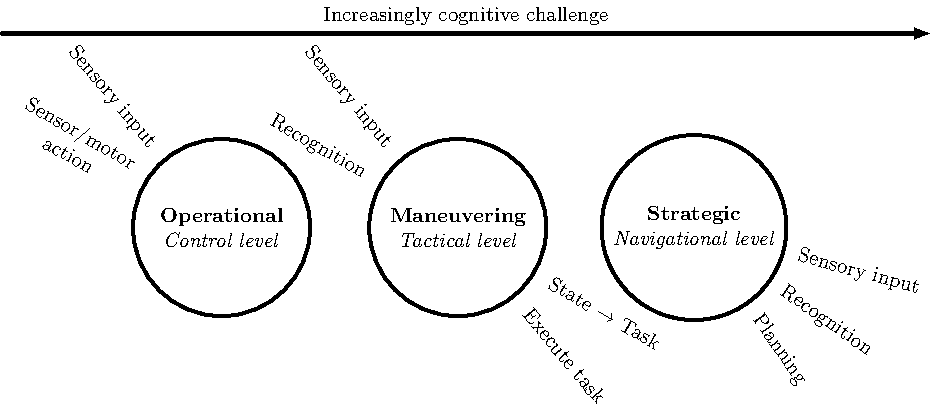
\includegraphics{three-layer-model-of-cognitive-tasks}
	\caption[Los tres niveles jerárquicos de conducción según~\cite{michon1985critical}]{Los tres niveles jerárquicos que describen la tarea de conducción según~\cite{michon1985critical}: \textit{estrategia} (i.e. las decisiones generales), la \textit{maniobra} (i.e. decisiones durante la conducción de más corto plazo) y \textit{control} (i.e. automatismos).}
	\label{fig:three-levels-of-human-driving}
\end{figure}

A pesar de que se trata de una clasificación subjetiva, es un modelo aampliamente aceptado dentro del área de los \gls{its}. Algunos estudios llegan incluso a definir intervalos de tiempo de razonamiento para las tareas de cada nivel, como por ejemplo~\cite{Alexiadis2004}, donde se llegan a proponer tiempos que separan unos niveles de otros: alrededor de \SI{30}{\second} para las tareas del nivel de planificación, entre \SI{5}{\second} a \SI{30}{\second} para las tareas de nivel táctico y por debajo de los \SI{5}{\second} para las tareas de control.

Otro modelo jerárquico de tres niveles muy referenciado en la literatura es el \textit{skill-rule-knowledge} de \cite{Rasmussen1986}, una generalización del modelo propuesto por \cite{michon1985critical} al comportamiento y razonamiento humano. Postula que éste se puede basar en \textbf{habilidades} (actividades completamente automatizadas de la forma \textit{percepción $\rightarrow$ ejecución}), \textbf{reglas} (situaciones familiares o estereotipadas de la forma \textit{percepción $\rightarrow$ reconocimiento de la situación $\rightarrow$ planificación $\rightarrow$ ejecución}) y \textbf{conocimiento} (actividades conscientes que implican resolución de problemas y toma de decisiones de la forma \textit{percepción $\rightarrow$ reconocimiento de la situación $\rightarrow$ toma de decisión $\rightarrow$ planificación de la ejecución}) que suelen ser necesarias en situaciones poco familiares). Algunos trabajos se basan en este modelo en lugar del de \cite{michon1985critical} como el presentado por \cite{Chaib-draa1994} donde abarca los tres niveles de abstracción representando en un escenario urbano tres tipos diferentes de situaciones: rutinaria, familiar y no familiar.

El comportamiento de un conductor al volante tiene una relación directa con el nivel de abstracción táctico. Se puede entender como el nivel encargado de planificar acciones a corto plazo para conseguir objetivos a corto plazo. Las tareas de control son automáticas e influyen poco o nada en la toma de deciones de tareas como \textit{cuánto acelerar en esta situación} o \textit{cuándo cambiar de carril}. Las tareas estratégicas están a un nivel más alto de abstracción (e.g. la ruta a seguir hasta mi destino) y tampoco afectan demasiado al comportamiento en situaciones concretas\sidenote{
	No obstante algunos trabajos han demostrado que en ocasiones la planificación de la ruta sí afecta a decisiones normalmente asociadas el nivel táctico como por ejemplo la preferencia de un conductor por uno u otro carril de la vía \cite{Wei2000, Toledo2003}.
}.

\newthought{Nuestro interés es el uso de agentes} como unidades en simulación. Después de todo trabajamos con \glsentrylongplsp{mas}. Sin embargo, y aunque en los trabajos más modernos exista una cierta predisposición hacia este paradigma, no todos los trabajos se basan en él. El auge de su uso coincide con el renacimiento de la \glsentrylongsp{ai}, alrededor de los años $90$, y los modelos que se describen en este apartado, sobre todo posteriores a esta fecha, se basan en este tipo de sistemas.

Las tipologías de agentes utilizadas es de todo tipo. Existen desde trabajos que explotan las características de los agentes reactivos (e.g. agentes que continuamente van realizando decisiones de control para mantenerse en la via \cite{Ehlert2001}) hasta aquellos que proponen complejos frameworks para definir comportamientos (e.g. cuatro unidades de funcionamiento interconectadas, \textit{percepción}, \textit{emoción}, \textit{toma de decisiones} y \textit{ejecución}, que gestionan el comportamiento inteligente del agente en cada situación \cite{al2001framework}).

La información que manejan estos agentes dentro de los simuladores suele limitarse a tipologías de vehículo (e.g. utilitarios o vehículos de grandes dimensiones) y magnitudes físicas (tamaño, velocidad máxima). Dependiendo del trabajo, algunos autores añaden más conocimiento a los agentes; por ejemplo, en \cite{hidas2002}, el autor incluye en los agentes, denominados \glspl{dvo} (otra denominación del concepto de \gls{dvu}), información adicional sobre el tipo de conductor y el nivel de conocimiento de la red de carreteras.

El resto del capítulo introducirá los modelos de comportamiento más conocidos y hará especial hincapié en el estado más reciente de modelos basados en técnicas de la \glsentrylongsp{ci}.

\section{Comportamientos modelados}

Las tareas que se realizan en el nivel táctico del comportamiento son aquellas orientadas a circular dentro del flujo de tráfico interactuando con éste. En la literatura, estas tareas se centran en dos clases generales de problema diferentes (figuras~\ref{fig:lane-selection-plus-merging} y~\ref{fig:acceleration-model-classes}): el de la \textbf{aceleración} y el del \textbf{cambio de carril}.

Los modelos de \textbf{aceleración} se ocupan de gestionar las alteraciones de la tasa de aceleración (positiva o negativa) en un entorno lineal como lo es un carril de tráfico.

\begin{figure}[t]
	\centering
	\begin{forest}
		for tree={
			align=center,
			parent anchor=south,
			child anchor=north,
			font=\sffamily,
			edge={thick, -{Stealth[]}},
			l sep+=10pt,
			edge path={
				\noexpand\path [draw, \forestoption{edge}] (!u.parent anchor) -- +(0,-10pt) -| (.child anchor)\forestoption{edge label};
			},
		}
		[Modelos de aceleración
			[\idx{free flow}]
			[\idx{approaching}]
			[\idx{car-following}]
			[\idx{emergency}]
			[\ldots]
		]
	\end{forest}
	\caption[Diferentes modelos de aceleración]{Tras la aparición de los modelos psico-físicos se comprobó que los umbrales en las percepciones y por tanto el comportamiento podía variar dependiendo de las situaciones. Por ello, el \textit{car-following} no era más que una entre diferentes clases o regímenes de aceleración. Algunos de los regímenes más usados en la literatura son \textit{free-flow}, \textit{car-following}, \textit{approaching}, y \textit{emergency}, aunque algunos autores definen nuevos regímenes, cada uno con sus límites de aplicación.}
	\label{fig:acceleration-model-classes}
\end{figure}

\begin{figure}[b]
	\centering
	\begin{forest}
		for tree={
			align=center,
			parent anchor=south,
			child anchor=north,
			font=\sffamily,
			edge={thick, -{Stealth[]}},
			l sep+=10pt,
			edge path={
				\noexpand\path [draw, \forestoption{edge}] (!u.parent anchor) -- +(0,-10pt) -| (.child anchor)\forestoption{edge label};
			},
		}
		[Modelos de cambio de carril
		[\idx{lane selection}]
		[\idx{gap acceptance}]
		[\idx{merging}]
		[\ldots]
		]
	\end{forest}
	\caption[Operaciones involucradas en el proceso de cambio de carril]{El cambio de carril se divide tradicionalmente en una operación que involucra dos pasos. La selección de carril (\textit{lane-selection}) al que cambiarse y la ejecución del cambio (\textit{merging}). En la operación de merging se suele involucrar otra operación denominada \textit{gap-acceptance}, aunque algunos autores la tratan como operación independiente. Otros autores pueden llegar a añadir opreaciones más especializadas.}
	\label{fig:lane-selection-plus-merging}
\end{figure}

El tráfico real, sin embargo, no está compuesto por un sólo carril, sino por varios. Los modelos de \textbf{cambio de carril} (figure~\ref{fig:lane-change-types}) tienen como objetivo identificar cuándo el conductor desea cambiar de carril y realizar dicho cambio, ya sea porque quiere mejorar su circulación (e.g. quiere realizar un adelantamiento) o porque su ruta lo requiere (e.g. está próxima la rampa de salida que quiere tomar en una autopista).

En la literatura los modelos de aceleración han sido mucho más estudiados que los de cambio de carril, entre otras cosas por la dificultad en la captura de los datos y, por tanto, por su escasez.

El estudio del comportamiento en los cambios de carril es muy interesante debido a que tiene efectos opuestos según la carga de tráfico de la vía en la que se ejecutan. Por un lado, si la carga de tráfico es de ligera, mejora la velocidad media del flujo de la vía. Sin embargo, según aumenta la carga de tráfico, los cambios de carril comienzan a afectar a éste en formas de ondas de choque (\cite{Sasoh2002, Jin2006}) e interferir incluso más que los modelos de \textit{\idx{car-following}} (\cite{Laval2006}).

\subsection{Nomenclatura}

Para no llevar a equívocos, en la figura \ref{fig:lane-representation-with-namings} se ilustran los actores típicos en una situación de tráfico junto con los nombres y su rol. A continuación los explicamos:

\begin{figure}[t]
	\missingfigure[figheight=4cm]{Ilustración estupenda y maravillosa de los vehículos en la vía y cómo están relacionados unos con otros.}
	\caption[Nomenclaturas a usar en los modelos de conducción]{Representación de los vehículos en una vía junto con la nomenclatura a usar durante el resto de la tesis.}
	\label{fig:lane-representation-with-namings}
\end{figure}

\begin{itemize}
	\item \textbf{Lag car}.
	\item \textbf{Lead car}.
\end{itemize}

\section{Modelado de conductores clásico}

Los primeros trabajos sobre modelos de conducción datan de comienzo de los años $50$ con estudios sobre el concepto denominado \textbf{\idx{car-following}}, acuñado por \cite{reuschel1950fahrzeugbewegungen}. Un vehículo está en una situación \idx{car-following} cuando su velocidad está condicionada por el vehículo que se encuentra frente a él. En el primer modelo concreto (\cite{Pipes1953}), el comportamiento responde a tratar de mantener un espacio variable en función de la velocidad.

Este modelo se puede considerar de una clase que denominaremos \textbf{mantenimiento de medida} dado que su objetivo es mantener constantemente una distancia segura, determinada a partir de la ecuación de la velocidad cuando el tiempo no baja de $1,02$ segundos. Otros trabajos trabajan con el mantenimiento de otras medidas como distancia relativa al parachoque delantero o trasero.

\marginnote{
	\textbf{El Modelo \glsentryshort{ghr}}, presentado en \cite{Chandler1958}, es el modelo más conocido antes de la introducción del modelo de Gipps. Desarrollado a finales de los años $50$ dentro de la \textit{General Motors} (por ello también se le conoce como modelo \gls{gm}), se caracteriza por el uso del concepto \textit{estímulo $\rightarrow$ respuesta}, donde la respuesta del vehículo (el cambio en la tasa de aceleración) es debida a la activación de un estímulo (la variación en la distancia con el vehículo delantero) tras pasar un tiempo de retardo $\tau$. Concretamente calcula el valor de la aceleración $a$ en un instante $t$ como:
	
	\begin{equation}
	a(t) = c v^m(t) \frac{\Delta v(t - \tau)}{\Delta x^l(t - \tau)}
	\label{eq:ghr-car-following-model}
	\end{equation}
	
	Siendo $t$ es el instante actual, $a(t)$ la aceleración del vehículo, $\delta v(t)$ y $\delta x(t)$ son la velocidad y distancia relativas al siguiente coche respectivamente, $v$ la velocidad del vehículo y $c$, $m$, $l$ y $\tau$ constantes, siendo ésta última el tiempo de reacción del conductor.
}

Más adelante, a finales de la decada se presentó el modelo \gls{ghr} (ver ecuación~\ref{eq:ghr-car-following-model}), el cual sirvió como base para el desarrollo de muchos modelos posteriores. Eset modelo dio origen a a una nueva clase de modelos de conducción, los de tipo \textbf{estímulo $\rightarrow$ respuesta}. 

\begin{figure}[t]
	\begin{center}
		\smartdiagramset{
			border color=none,
			back arrow disabled=true,
			text width=2.4cm,
			module x sep=3.5cm
		}
		\smartdiagram[flow diagram:horizontal] {
			Mantenimiento de medidas,
			estímulo~/ respuesta,
			psico-físicos
		}
		\caption[Evolución de los tres tipos generales de modelo de \textit{car-following}]{Evolución de los tres tipos generales de modelo de \textit{car-following}: mantenimiento de medidas, estímulo$\rightarrow$respuesta y psico-físicos. Con la llegada de los psico-físicos se vio que \textit{car-following} no era más que uno de tantos regímenes distintos dentro de los modelos de aceleración.}
		\label{fig:car-following-there-different-models}
	\end{center}
\end{figure}

En realidad los modelos \textit{estímulo $\rightarrow$ respuesta} son la evolución lógica de los modelos anteriores, donde se pasa de un cálculo de velocidad en función de la distancia (u otra medida) a un sistema de control donde la variable a controlar es la aceleración en función de uno o varios estímulos de entrada, además con un retardo simulando el tiempo de reacción. Algunas modificaciones sobre el algoritmo original son la asimetría en la tasa de cambio de aceleración y deceleración \cite{Gazis1959} o la inclusión del efecto de segundos coches delanteros \cite{Bexelius1968}.

Los métodos de estas dos clases tienen un problema principal: suponen que el conductor es capaz de percibir incluso el más ínfimo cambio en las variables observadas, cuando la realidad no es así. Por ello, a mediados de los años $70$ apareció una nueva clase de modelos de \textit{\idx{car-following}}, denominados posteriormente como \textbf{psicofísicos} \cite{wiedemann1974simulation}, donde se introduce el concepto de \textit{\idx{umbral perceptual}} como solución a dicha limitación. El \textit{umbral perceptual} de una medida es el límite a partir del cual se percibe un cambio en dicha medida. Mediante su uso, las acciones de los vehículos se limitan únicamente a los cambios \textbf{perceptibles} en los coches delanteros.

A finales de la década, en $1978$, se cumplió otro hito en el desarrollo de modelos de conducción. \cite{Sparmann1978} define el primer modelo de cambio de carril, inspirándose en las clases de modelo psicofísico. El verdadero interés de este modelo es que sentó las bases de dos conceptos que perduran hoy en día. El primero, la diferenciación entre cambio a carriles rápidos y lentos\sidenote{
	En \cite{Sparmann1978} el autor entiende la derecha como el carril lento y la izquierda como el carril rápido, y es como se entiende dentro del contexto de esta tesis. Sin embargo en otros países esta correspondencia es al revés.
}. El segundo, la diferenciación entre la selección de carril o \textit{\idx{lane-selection}} y la ejecución del cambio o \textit{\idx{merging}}.

\newthought{La viabilidad en un cambio de carril} se determina haciendo uso de modelos denominados \textit{\idx{gap acceptance}}, donde los vehículos calculan si caben o no en un determinado hueco y actuan en consecuencia.

En su origen los modelos de \textit{\idx{gap acceptance}} se desarrollaron para resolver situaciones en intersecciones e incorporaciones. En la actualidad son los modelos usados tras seleccionar el cambio de carril y antes de ejecutar físicamente el cambio, y dependiendo del modelo, es incluido como operación dentro de uno u otro.

En general se basan en una fórmula que determina si el cambio es viable o no en función de una serie de parámetros entre los que se incluye el hueco del carril destino. En la ecuación~\ref{eq:gap-acceptance-model} se describe el modelo típico de un modelo de \textit{\idx{gap accceptance}}. 

\marginnote{
	El modelo típico del \textbf{\idx{gap acceptance}} responde a la ecuación~\ref{eq:gap-acceptance-model}, donde en un momento $t$, el cambio a un carril $l$ es viable ($f_{g_l}(t) = 1$) o no ($f_{g_l}(t) = 0$) dependiendo de si el espacio en el carril destino $g_l(t)$ es mayor o menor que un \enquote{hueco crítico} (en inglés \idx{critical gap}) $g^{crit}_l(t)$.
	
	\begin{equation}
	f_{g_l}(t) = \twopartf {0} {g_l(t) < g^{crit}_l(t)} {1} {g_l(t) \geq g^{crit}_l(t)}
	\label{eq:gap-acceptance-model}
	\end{equation}
	
	Por otro lado, existen autores que definen factores de influencia que modifican el modelo típico. Algunos ejemplos de factores pueden ser la velocidad absoluta del vehículo (\cite{Gipps1986, Ahmed1996}),el tipo de cambio (\gls{mlc} o \gls{dlc}, usado en \cite{Ahmed1999, Toledo2007}), la relativa con los vehículos delantero y trasero del carril destino (\cite{Ahmed1999}) o incluso el peso de encontrarse o no en una situación de cooperación (\cite{Ahmed1999, Hidas2002}).
}

\newthought{con los modelos psicofísicos} se llegó a la conclusión que no todas las situaciones eran iguales, sino que en función del entorno y el momento los umbrales podían variar, y que el \textit{\idx{car-following}} no era sino un subtipo más de una clase más amplia que se definió como \textit{modelos de aceleración} (figura~\ref{fig:acceleration-model-classes}).

Debido a eso y a la irrupción de los modelos de cambio de carril, los posteriores modelos y \textit{frameworks} desarrollados se componen de dos o más submodelos que responden a diferentes umbrales. Sin embargo, esto provoca que los modelos desarrollados sean más complejos ya que, cuantos más regímenes se tratan de agrupar en un mismo modelo, más aumenta el número de factores a generalizar y ajustar.

\newthought{El trabajo de Gipps} es uno de los primeros modelos que agrupa varios regímenes distintos (concretamente \textit{\idx{car-following}} y \textit{\idx{free-flow}}) \cite{Gipps1981}. Sin embargo consideramos más interesante su posterior trabajo, \cite{Gipps1986} ya que puede considerarse como la primera solución para el cambio de carril.

Introduce el concepto de que los cambios de carril obedecen a diferentes motivaciones. Por un lado, los cambios pueden ser \textbf{obligatorios} (denominado en la literatura como \gls{mlc}) cuando los vehículos se ven obligados a abandonar el carril que ocupan. Por otro lado, pueden ser \textbf{discrecionales} cuando el cambio obedece a motivaciones más relacionadas con la mejora del confort o de la situación actual de conducción (ver figura~\ref{fig:lane-change-mandatory-vs-discretional}).

\begin{figure}[t]
	\missingfigure[figheight=4cm]{Dos ilustraciones, una con un cambio de carril obligatorio (que se acabe el carril por ejemplo) y otro discrecional (que se vea un vehículo lento como un camión y el coche adelantando).}
	\caption[Ejemplo de cambio de carril obligatorio frente a cambio de carril discrecional]{Los cambios de carril se clasifican como aquellos necesarios para continuar con la conducción (obligatorios) y aquellos útiles para mejorar la situación de conducción (discrecionales).}
	\label{fig:lane-change-mandatory-vs-discretional}
\end{figure}

En su modelo, Gipps propone un modelo para el cambio de carril al aproximarse a un cambio de dirección. Dicho modelo identifica tres distancias que caracterizan el comportamiento del conductor en función de cómo de lejos está dicho punto: (i) \textbf{lejos}, en el que no existe condicionamiento en la decisión de cambio de carril, (ii) \textbf{medio}, donde el conductor empieza a ignorar los cambio que dan ventaja de velocidad si no hacia carriles distanciados del de salida y (iii) \textbf{cerca} donde los vahículos deben estar en el carril de cambio de salida.

Otro concepto que incluye el modelo de Gipps y que exporta a modelos posteriores de cambio de carril\index{lane-changing} es el de ampliar el número de \index{critical-gap}\textit{critical gaps} a más de un hueco: las distancias hasta el vehículo delantero y hasta el vehículo trasero, forzando a que durante el proceso de \textit{\idx{gap-acceptance}} las condiciones de ambos huecos tengan que ser aceptables.

Posteriormente, en \cite{wiedemann1992microscopic} se desarrolla un framework similar pero teniendo en cuenta los cambios a carriles lentos (para representar, por ejemplo, obstrucciones como accidentes o un vehículo lento) y a carriles rápidos (para situaciones como condiciones de la ruta). Además el autor incluye un modelo para influir en su desempeño en función del entorno actual (las características de los vehículos de alrededor) y el entorno potencial (la estimación de las características del entorno en momentos posteriores).

\begin{figure}[t]
	\missingfigure[figheight=4cm]{Tres ilustraciones, una para cada caso de lejos, medio y cerca..}
	\caption[Efecto de la distancia en el tipo de cambio de carril según el modelo de \cite{Gipps1986}]{En el modelo de \cite{Gipps1986}, la distancia al punto (i.e. cerca, media distancia y lejos) determina el grado de obligatoriedad del cambio.}
	\label{fig:lane-change-type-depending-on-the-distance}
\end{figure}

\marginnote{
	En el trabajo de \cite{wiedemann1992microscopic} se proponen hasta cuatro clases diferentes de modelos de aceleración en función de las posiciones y velocidades relativas entre el vehículo sujeto y el siguiente: (i) \textbf{free-flow}, donde el comportamiento no se ve afectado por el del vehículo delantero), (ii) \textbf{car-following}, donde el comportamiento sí se ve influenciado por el vehículo delantero, obligando a disminuir la velocidad deseada en el conductor en cuestión, (iii) \textbf{approaching}, stuación intermedia entre las dos anteriores y (iv) \textbf{emergency}, donde la situación es crítica (e.g. colisión inminente) obligando, normalmente, a respuestas extremas.
	
	Esto es sólo un ejemplo, y diferentes autores identifican diferentes situaciones dependiendo del alcance del trabajpo como por ejemplo el \textit{close-following} o el \textit{stop-and-go} \cite{Toledo2003, Liu2013}).
}

El modelo de Gipps sin embargo, sufre de dos problemas clave. Muchos de estos problemas fueron heredados por posteriores trabajos que basaban su funcionamiento en éste.

\newthought{Un cambio de carril no sólo involucra} al conductor que lo ejecuta. En \cite{Hidas2002}, el autor resalta el problema de que, en situaciones de congestión, el cambio ha de ser o bien forzado o bien a través de colaboración; en caso contrario, los vehículos no abandonarán el carril congestionado.

Uno de los primeros trabajos en abordar el comportamiento colaborativo es el de \cite{Fritzsche1994}. En éste, se describe un modelo de microsimulación para analizar cuellos de botella (e.g. un accidente donde se bloquea uno de los carriles). Los autores describen el problema pero no consideran la modificación de los modelos en cambio de carril. \cite{Yang1996} sin embargo presenta un entorno de simulación (\gls{mitsim}) que introduce, entre otros, un modelo de cambio de carril en el que se habla específicamente de comportamiento colaborativo. Introducen el concepto de función de cortesía (\textit{\idx{courtesy yielding function}}) la cuál afecta al modelo de \textit{\idx{car-following}} de un vehículo cuando otro intenta incorporarse al carril. Sin embargo, los detalles de dicho proceso no están especificados en el artículo.

\begin{figure}
	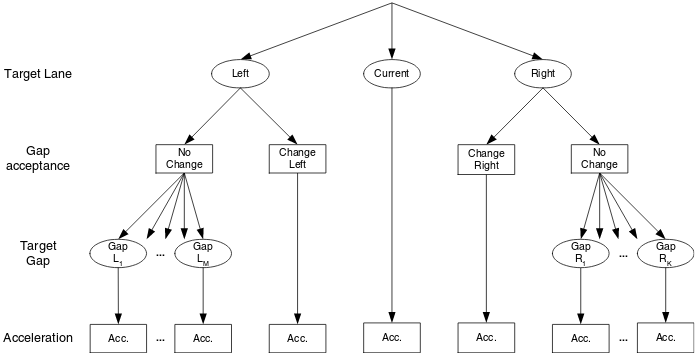
\includegraphics{toledo-2007-behavior-model-tree}
	\caption[Estructura del modelo de comportamiento propuesto por \cite{Toledo2007}]{Estructura del modelo de comportamiento de los vehículos propuesto por \cite{Toledo2007}. Este modelo se basa en el concepto de \enquote{objetivo a corto plazo} para elaborar un \enquote{plan a corto plazo} apoyándose, para ello, en un arbol de decisión. Aunque mantiene la clasificación, es probabilístico y existe opción de realizar un \gls{dlc} en lugar de un \gls{mlc} aún en situaciones donde acciones de ambas clases se activen. Para ello implementa agentes basados en utilidad donde ésta se calcula teniendo en cuenta cada uno de los nodos en un árbol de decisión. Fuente: \cite{Toledo2007}.}
	\label{fig:toledo-2007-behavior-model-tree}
\end{figure}

\newthought{Además, al usar árboles secuenciales}, los factores son evaluados uno detrás de otro hasta encontrar una situación favorable, en cuyo caso el resto de factores no son evaluados. Por ejemplo, tal y como está formado el modelo de Gibbs, y algunos basados en éste como \cite{Hidas2002}, un \gls{mlc} inhibe cualquier posibilidad de realizar un \gls{dlc} independientemente de la utilidad de ambos. Para evitar esta limitación, algunos autores hacen uso de técnicas como modelos probabilísticos. Ejemplos de avances en esta línea de trabajo pueden ser \cite{Toledo2003, Toledo2007, Wei2000} (figura~\ref{fig:toledo-2007-behavior-model-tree}).

\section{Modelado basado en \glsentrylongsp{ci}}

Desde mediados de los años $90$ empezó a crecer el interés por aplicar la \glsentrylongsp{ai} a los \gls{its}. Hay dos razones por las que esto es así: la primera, los éxitos cosechados por la \glsentrylongsp{ci}, los cuales atrayeron a investigadores de multitud de áreas incluida ésta. La segunda, el rápido desarrollo de la tecnología\sidenote{
	La tecnología es cada vez más barata, más precisa y con más funcionalidades. En la última década hemos vivido una explosión de dispositivos de todo tipo: teléfonos y relojes con GPS, acelerómetros y giroscopio, ordenadores completamente funcionales del tamaño de una moneda, sensores RADAR y LIDAR para uso amateur además de profesional y así un largo etcétera.
}, que posibilita la existencia de conjuntos de datos masivos con la capacidad de explotarlos y aprender de ellos.

Algunos autores (\cite{Zhang2011}) se atreven a afirmar incluso que el futuro de las \gls{its} son las técnicas de la \gls{ci}, y que los resultados que se puedan cosechar de técnicas basadas en el desarrollo convencional de sistemas es marginal comparado con las que se obtendrán con el nuevo enfoque.

Dentro de las \gls{its}, las áreas de aplicación de la \gls{ci} se centran en los siguientes conceptos: \textbf{reconocimiento de patrones}, \textbf{caracterización de conductores} y \textbf{modelado de conductores}. Es necesario mencionar que aunque se trate de áreas distintas, éstas suelen retroalimentarse, y es difícil encontrar estudios que se centren en una única área sin tocar el resto (figura~\ref{fig:main-applications-of-ci-in-its}). Por ello, aunque nuestro interés pueda centrarse en el modelado de conductores, es necesario conocer el estado de las demás áreas.

\begin{figure}[t]
	\centering
	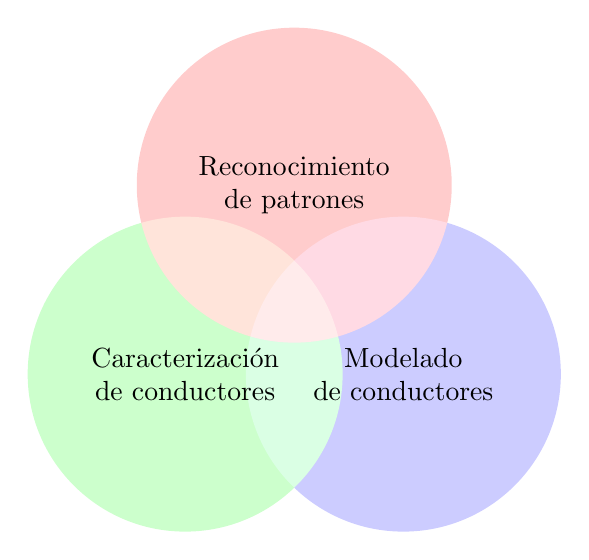
\begin{tikzpicture}
	\begin{scope}[blend group = soft light]
	\fill[red!20!white]   ( 90:1.6) circle (2);
	\fill[green!20!white] (210:1.6) circle (2);
	\fill[blue!20!white]  (330:1.6) circle (2);
	\end{scope}
	\node at ( 90:1.6) [align=center] {
		Reconocimiento\\ de patrones
	};
	\node at ( 210:1.6) [align=center] {
		Caracterización\\ de conductores
	};
	\node at ( 330:1.6) [align=center] {
		Modelado\\ de conductores
	};
	\end{tikzpicture}
	\caption[Principales areas de aplicación de la \glsentrylongsp{ci} en los \gls{its}]{Las principales areas de aplicación de la \glsentrylongsp{ci} en los \gls{its} son el reconocimiento de patrones, la caracterización de conductores y la modelización de los mismos. Aunque son áreas de aplicación distintas, los estudios en general tienden a solaparse. Por ejemplo, las técnicas de reconocimiento de patrones pueden usarse como forma de extracción de características para una caracterización de conductores y a su vez esta caracterización puede usarse como base para su modelado.}
	\label{fig:main-applications-of-ci-in-its}
\end{figure}

\begin{itemize}
	\item En el \textbf{reconocimiento de patrones} las técnicas suelen trabajar en los temas de extracción de características y de predicción de comportamientos. La cantidad de datos que se pueden generar en un coche es tal que el trabajo a través de información en curdo es inviable (no digamos ya cuando los datos son extraídos de una flota de vehículos).
	\item La \textbf{caracterización de conductores} es interesante debido a que permite la identificación de perfiles de conducción y su clasificación de acuerdo a indicadores extraídos de su manera de conducir.
	\item El \textbf{modelado de conductores} nos permite la reproducción de coómportamientos en simulación.
\end{itemize}

Las técnicas de \gls{ci} más utilizadas en el modelado de conductores son las \glsentrylongplsp{ann} y la \glsentrylongsp{fl}. Es comprensible dado que las primeras son una de las técnicas principales en la rama del \glsentrylongsp{ml}, y la segunda por ser una manera sencilla y cercana a la manera de razonar del ser humano.

Sólo por la propia naturaleza de las técnicas, los modelos incluyen siempre más de un único comportamiento: al ser entrenados con datos de conductores reales y manejar la información con incertidumbre, \enquote{aprenden} a comportarse en diferentes regímenes (e.g. \textit{\idx{free-flow}}).

\newthought{Las \glsentrylongplsp{ann}} fueron el punto de entrada de la \gls{ci} en la modelización de conductores. Los perceptrones multicapa y sus nuevas técnicas de entrenamiento se habían convertido en la nueva solución universal para todo aquel problema del que se dispusiese de datos.

\begin{figure}
	\missingfigure[figheight=4cm]{Creo que una ilustración pequeña aquí de un controlador difuso y una red neuronal quedaría genial.}
	\caption[La inexactitud se tiene en cuenta en los modelos de la \glsentrylongsp{ci}]{Al trabajar con métodos como las \glsentrylongplsp{ann} o la \glsentrylongsp{fl}, la inexactitud y la incertidumbre son ciudadanos de primera clase y forman parte de los modelos.}
	\label{fig:ann-and-fl-work-with-uncertainty}
\end{figure}

Las \gls{ann} se han aplicado mucho sobre el campo de los \glspl{its} en general, no sólo en modelado de conductores sino en prácticamente todos los aspectos como la clasificación de conductores \cite{DiazAlvarez2014}, la conducción autónoma \cite{huval2015empirical} o la predicción (\cite{Dougherty1993, chan2012neural} entre muchos otros.

El primer trabajo de la literatura sobre la aplicación de \glspl{ann} al modelado de conductores es \cite{Fix1990}, donde los autores desarrollan un controlador para imitar el comportamiento de un conductor.

En la misma década, en \cite{Hunt1994} se desarrolló uso de \gls{ann} aplicadas al entorno del vehículo para identificar el entorno y determinar cuándo y cómo realiza el conductor un cambio de carril.

Los modelos hasta el momento hacen uso de datos extraídos de conductores reales pero desde entorno de simulación. El primer trabajo en usar datos reales de vehículos instrumentados para este cometido es \cite{Jia2003}. A partir de las entradas correspondientes a velocidad relativa, espacio relativo, velocidad y velocidad deseada (para ello, clasifican al conductor de agresivo, normal, conservador) determinan la aceleración/deceleración del vehículo. No lo aplican a ningún simulador, sólo que los valores se ajustan. Otros trabajos similares son \cite{Panwai2007, Khodayari2012}.

El trabajo de \cite{Simonelli2009} también se apoya en datos extraídos de entornos reales. El interés de este estudio radica en que es el primero en realizar una comparativa entre el desempeño de una arquitectura \textit{\idx{fast-forward}} (e.g. perceptrón multicapa) frente a una \idx{recurrente} (e.g. red de Elman). El por qué del uso de redes recurrentes es por su capacidad de reconocer patrones dinámicos, los cuales son de esperar en este tipo de comportamientos.

\newthought{El primer uso de la \glsentrylongsp{fl}} fue contemporáneo al de las \gls{ann}, y también aplicada a un modelo de \textit{\idx{car-following}}. Después de todo los modelos psicofísicos aparecieron debido a que la percepción del conductor no es absoluta, sino imprecisa.

Estos modelos parten de la hipótesis de que la información que maneja el conductor a la hora de tomar decisiones proviene de un análisis no demasiado detallado de la situación que le rodea; es decir, la percepción y el comportamiento humanos son estímulos percibidos de manera aproximada. Por tanto, el resultado debe ser fruto de un proceso de razonamiento que tenga en cuenta esa imprecisión en los estímulos, y la lógica difusa es ideal para modelar la incertidumbre del mundo real y por tanto de las percepciones de los conductores.

\cite{Kikuchi1992} es el primer trabajo documentado sobre el tema. En él, los autores aplicaron la lógica difusa sobre un modelo de aceleración de tipo \textit{\idx{car-following}}. Utilizaron el modelo \gls{ghr} (Ecuación~\ref{eq:ghr-car-following-model}) como base y determinaron las entradas al modelo como valores de pertenencia a conjuntos difusos. Las entradas del modelo eran las distancia y velocidad relativa entre el vehículo modelado y el delantero y la variación en la aceleración del vehículo delantero. Como salida, el cambio en la tasa de aceleración sobre el vehículo modelado.

\cite{McDonald1997, Wu2003} desarrollaron del modelo \gls{flowsim} con similares características pero incluyendo el comportamiento de cambio de carril, además en dos categorías: al carril \textbf{lento} (principalmente para evitar incordiar a los vehículos que se aproximan por detrás a velocidades superiores, usan dos variables, presión del vehículo trasero y satisfacción en el gap del carril destino) y al \textbf{rápido} (para ganar velocidad, variables: velocidad ganada con el cambio y oportunidad, es decir, seguridad y confort con el cambio).

Los modelos hasta el momento se basaban en conjuntos difusos y reglas definidos \textit{ad-hoc}. En \cite{Chakroborty2003} se introduce el concepto de personalización, ajustando los conjuntos difusos de las variables de entrada y salida a valores extraídos de conductores reales. Este ajuste se realiza mediante la representación del controlador difuso como red neuronal y posterior ajuste mediante entrenamiento de dicha red (\textit{\idx{back-propagation}}). A este trabajo le siguen muchas otras aproximaciónes \textit{\idx{neuro-fuzzy}} como \cite{Ma2004, Zheng2005}

\begin{marginfigure}
	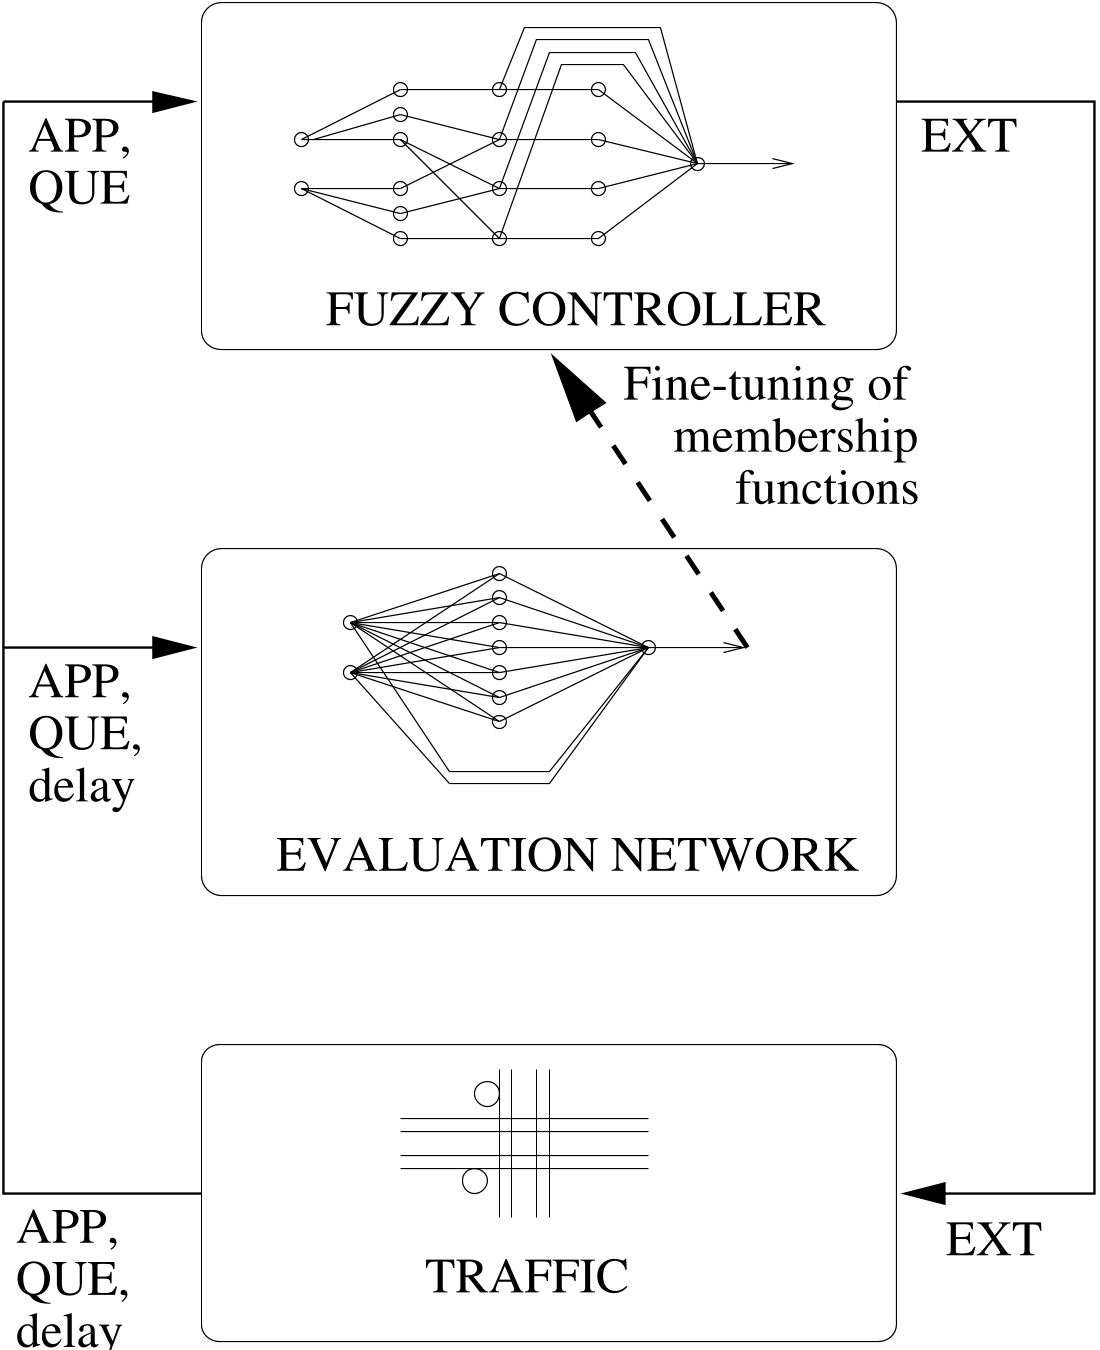
\includegraphics{neuro-fuzzy-in-its}
	\caption[Ejemplo de aproximación \textit{neuro-fuzzy} al control de señales de tráfico]{Un ejemplo de aproximación \textit{neuro-fuzzy}, en este caso aplicado al control de señales de tráfico. El \glsentrylongsp{fcs} se implementa como una \glsentrylongsp{ann} de tipo \textit{feed-forward} en lugar de con una representación tradicional. Además, el sistema completo lleva integrado un subsistema basado en también en \glsentrylongplsp{ann} \textit{feed-forward} que ajusta las funciones de pertenencia a trabés de enrtenamiento por refuerzo. Fuente: \cite{bingham2001reinforcement}}
	\label{fig:neuro-fuzzy-in-its}
\end{marginfigure}

Más adelante, en \cite{Das2009}, dentro de su simulador \gls{aasim} añaden los conceptos de \gls{mlc} y \gls{dlc} a los comportamientos de cambos de carril. En \gls{mlc} las reglas tienen en cuenta la distancia al siguiente punto característico (e.g. una salida) y el número de cambios de carril necesarios. En \gls{dlc} deciden si cambiar o no basándose en el nivel de satisfacción del conductor y en el nivel de congestión en los carriles adjacentes\sidenote{
	Este trabajo se apoya en trabajos anteriores que separan las jerarquías en situaciones de \gls{mlc} y \gls{dlc} como \cite{Yang1996, Halati1997, Hidas2002}. Estos trabajos, no obstante, no pertenecen al área de la \gls{ci}.
}.

\newthought{Las \glsentrylongplsp{ann} y la \glsentrylongsp{fl} no son} las únicas técnicas usadas para determinar comportamientos en conductores.

Por ejemplo, en \cite{maye2011bayesian} se presenta un modelo no supervisado, online y basado en redes bayesianas donde se infiere el comportamiento del conductor haciendo uso de una \gls{imu} y una cámara. De la \gls{imu} se extraen datos que se separan en fragmentos para luego relacionarlos con las imágenes obtenidas de la cámara. Otro trabajo similar pueden ser \cite{van2013driver} el cual se apoya también en la segmentación de los datos extraídos de una \gls{imu} pero con técnicas distintas (concretamente \textit{clustering} basado en \gls{svm} y en $k$-medias) y sin cámara.

En~\cite{bando2013unsupervised} describen otro modelo no supervisado, éste offline, basado en un modelo bayesiano no paramétrico para la clusterización, combinándolo con un modelos supervisado (\gls{lda}) para la clusterización a más alto nivel. El trabajo de \cite{bender2015unsupervised} usa una aproximación similar pero sin la segunda clusterización.

Otra aproximación es el de los \glspl{hmm}. Por ejemplo, los trabajos \cite{Kuge2000,sekizawa2007modeling} aplican entrenamiento supervisado sobre estos modelos para reconocer los eventos que están provocando los conductores (concretamente cambiando de un carril a otro). En \cite{Hou2011} van un paso más allá desarrollando un modelo capaz de estimar si el conductor va a realizar un cambio a la derecha o a la izquierda a partir del ángulo de giro del volante (con una precisión de $~0.95$ en una ventana temporal de $1.5$ segundos y de $~0.83$ en una ventana de $5$ segundos).

Por último, \cite{Aghabayk2013} presenta un modelo basado en \gls{lolimot} que son similares a una aproximación \textit{\idx{neuro-fuzzy}} del comportamiento. Intenta incorporar imperfecciones perceptuales en un modelo de \textit{\idx{car-following}}.

\newthought{Estas técnicas no sólo se usan para} modelar comportamientos complejos o modelos enteros. Algunos trabajos se ocupan de características o aspectos de un modelo concreto. Por ejemplo, los trabajos \cite{Hatipkarasulu2002, zheng2013} se ocupan exclusivamente del cálculo de tiempo de respuesta del conductor en modelos de \textit{\idx{car-following}}, el primero con controladores difusos y el segundo con \glspl{ann}.

\section{Papers a añadir o al menos relevantes}

Analysis of Recurrent Neural Networks for Probabilistic Modeling of Driver Behavior (de Morton J, Wheeler T, Kochenderfer M). Explora redes recurrentes para estudiar modelos de aceleración.
Review of microscopic lane-changing models and future research opportunities. Su propio nombre dice de qué va.
A review of intelligent driving style analysis systems and related artificial intelligence algorithms. Este lo mismo sirve para completar algún hueco que haya quedado en el estado del arte. Es relativamente reciente.
